\section{\src{comp_caldyn_horiz}}

\subsection{Description}

Kernel \src{comp_caldyn_horiz} is taken from the original subroutine
\src{compute_caldyn_horiz} in \DYNAMICO.
%
This subroutine is originally defined in module \src{caldyn_gcm_mod}.
%
This module defines subroutine \src{caldyn}, which is the main
subroutines for dynamics part of the model, and several sub-subroutines
for various terms in the governing equation, such as potential
vorticity, geopotential, etc.
%
This subroutine calculates several horizontal terms, including mass
flux, Bernouilli term, etc.


\subsection{Discretization and code}

\autoref{l:definition_comp_caldyn_horiz} shows the definition part of this subroutne,
and \autoref{f:pad_comp_caldyn_horiz_1}, \ref{f:pad_comp_caldyn_horiz_2}, \ref{f:pad_comp_caldyn_horiz_3}
show the PAD of this.


\begin{LstF90}[%
caption={Definition part of \src{compute_caldyn_horiz}},%
label={l:definition_comp_caldyn_horiz}%
]
  SUBROUTINE compute_caldyn_horiz(u,rhodz,qu,theta,pk,geopot, hflux,convm, dtheta_rhodz, du)
  USE icosa
  USE disvert_mod
  USE exner_mod
  USE trace
  USE omp_para
  IMPLICIT NONE
    REAL(rstd),INTENT(IN)  :: u(iim*3*jjm,llm)    ! prognostic "velocity"
    REAL(rstd),INTENT(IN)  :: rhodz(iim*jjm,llm)
    REAL(rstd),INTENT(IN)  :: qu(iim*3*jjm,llm)
    REAL(rstd),INTENT(IN)  :: theta(iim*jjm,llm)  ! potential temperature
    REAL(rstd),INTENT(INOUT) :: pk(iim*jjm,llm) ! Exner function
    REAL(rstd),INTENT(IN)  :: geopot(iim*jjm,llm+1)    ! geopotential

    REAL(rstd),INTENT(INOUT) :: hflux(iim*3*jjm,llm) ! hflux in kg/s
    REAL(rstd),INTENT(INOUT) :: convm(iim*jjm,llm)  ! mass flux convergence
    REAL(rstd),INTENT(INOUT) :: dtheta_rhodz(iim*jjm,llm)
    REAL(rstd),INTENT(INOUT) :: du(iim*3*jjm,llm)

    REAL(rstd) :: cor_NT(iim*jjm,llm)  ! NT coriolis force u.(du/dPhi)
    REAL(rstd) :: urel(3*iim*jjm,llm)  ! relative velocity
    REAL(rstd) :: Ftheta(3*iim*jjm,llm) ! theta flux
    REAL(rstd) :: berni(iim*jjm,llm)  ! Bernoulli function

    INTEGER :: i,j,ij,l
    REAL(rstd) :: ww,uu
\end{LstF90}

Where \src{u}, \src{rhodz}, \src{qu}, \src{geopot} are wind velocity on the edge,
mass, potential vorticity on the edge, and geopotential, respectively.
\src{pk}, \src{hflux}, \src{convm}, \src{dtheta_rhodz}, \src{du} are Exner function,
horizontal mass flux on the edge, mass flux convergence,
time derivative of the mass-weighted potential temperature,
and time derivative of wind velocity on the edge.
%
Local arrays \src{cor_NT}, \src{urel}, \src{Ftheta}, \src{berni} are
Coriolis's force, relative velocity, potential temperature flux and
Bernoulli function, respectively.
%
All of these arrays are two dimensional.
%
First dimension is for horizontal index, and the size depends on the point
where the variable is defined, since \DYNAMICO adopts C-grid.
%
Second dimension is for vertical index, and the size is \src{llm},
except \src{llm+1} for \src{geopot} that is defined on the half level in
vertical, while others are defined on the full level.


This subroutine is relatively long, and is able to be split by three
sections.
%
In the first section (\autoref{f:pad_comp_caldyn_horiz_1}), there is one $l$-loop
and two $ij$-loop in it.
%
The first one calculates mass flux \src{hflux} and potential
temperature flux \src{Ftheta} at the edge of each control volume.
%
The second loop calculates convergence of mass flux \src{convm}
and convergence of potential temperature flux \src{dtheta_rhodz}.

\begin{figure}[tbp]
\centering
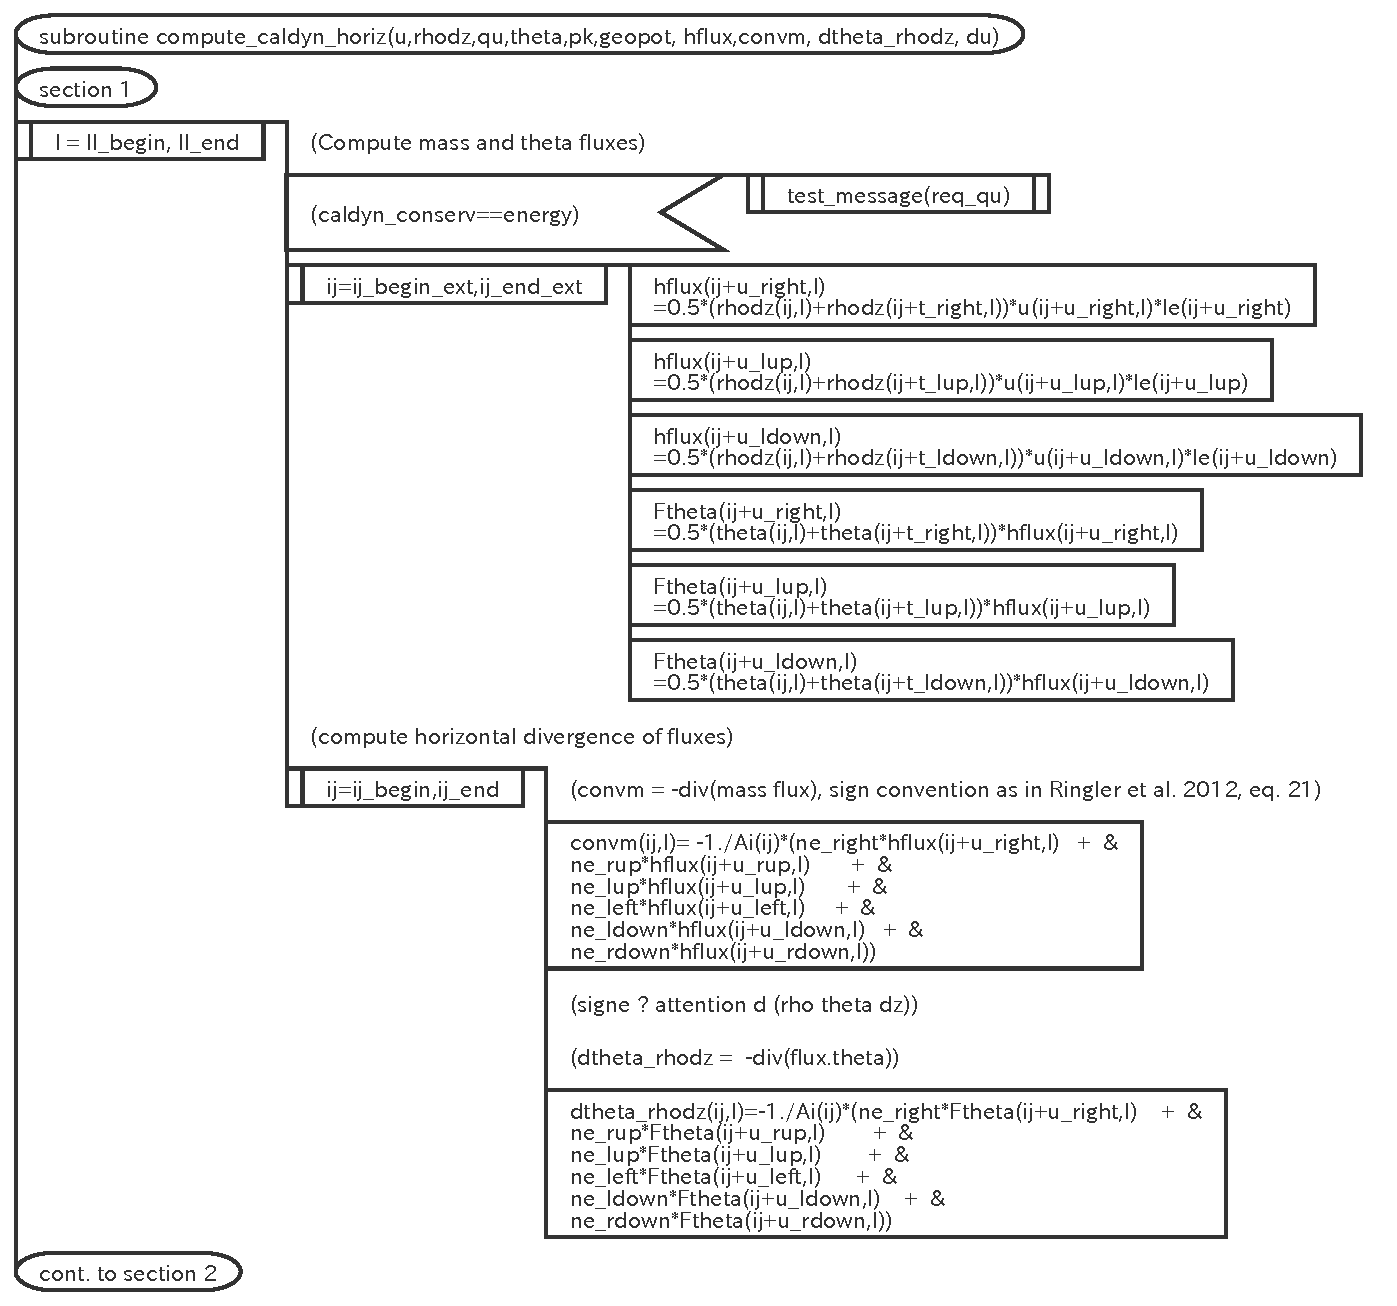
\includegraphics[scale=.6]{figs/caldyn_horiz_sec1.pdf}
 \caption{PAD of \src{compute_caldyn_horiz(1)}}\label{f:pad_comp_caldyn_horiz_1}
\end{figure}


The second section (\autoref{f:pad_comp_caldyn_horiz_2}) calculates potential
vorticity contribution to \src{du} based on the TRiSK scheme
\citep{Ringler:2010:UAE:1749635.1750220}.
%
Here \src{wee} is interpolating weight, prepared in module
\src{geometry} in original \DYNAMICO.
%
Note that since \src{caldyn_conserv} is set as
\src{energy} in this kernel program, second choice of CASE is selected.


\begin{figure}[tbp]
\centering
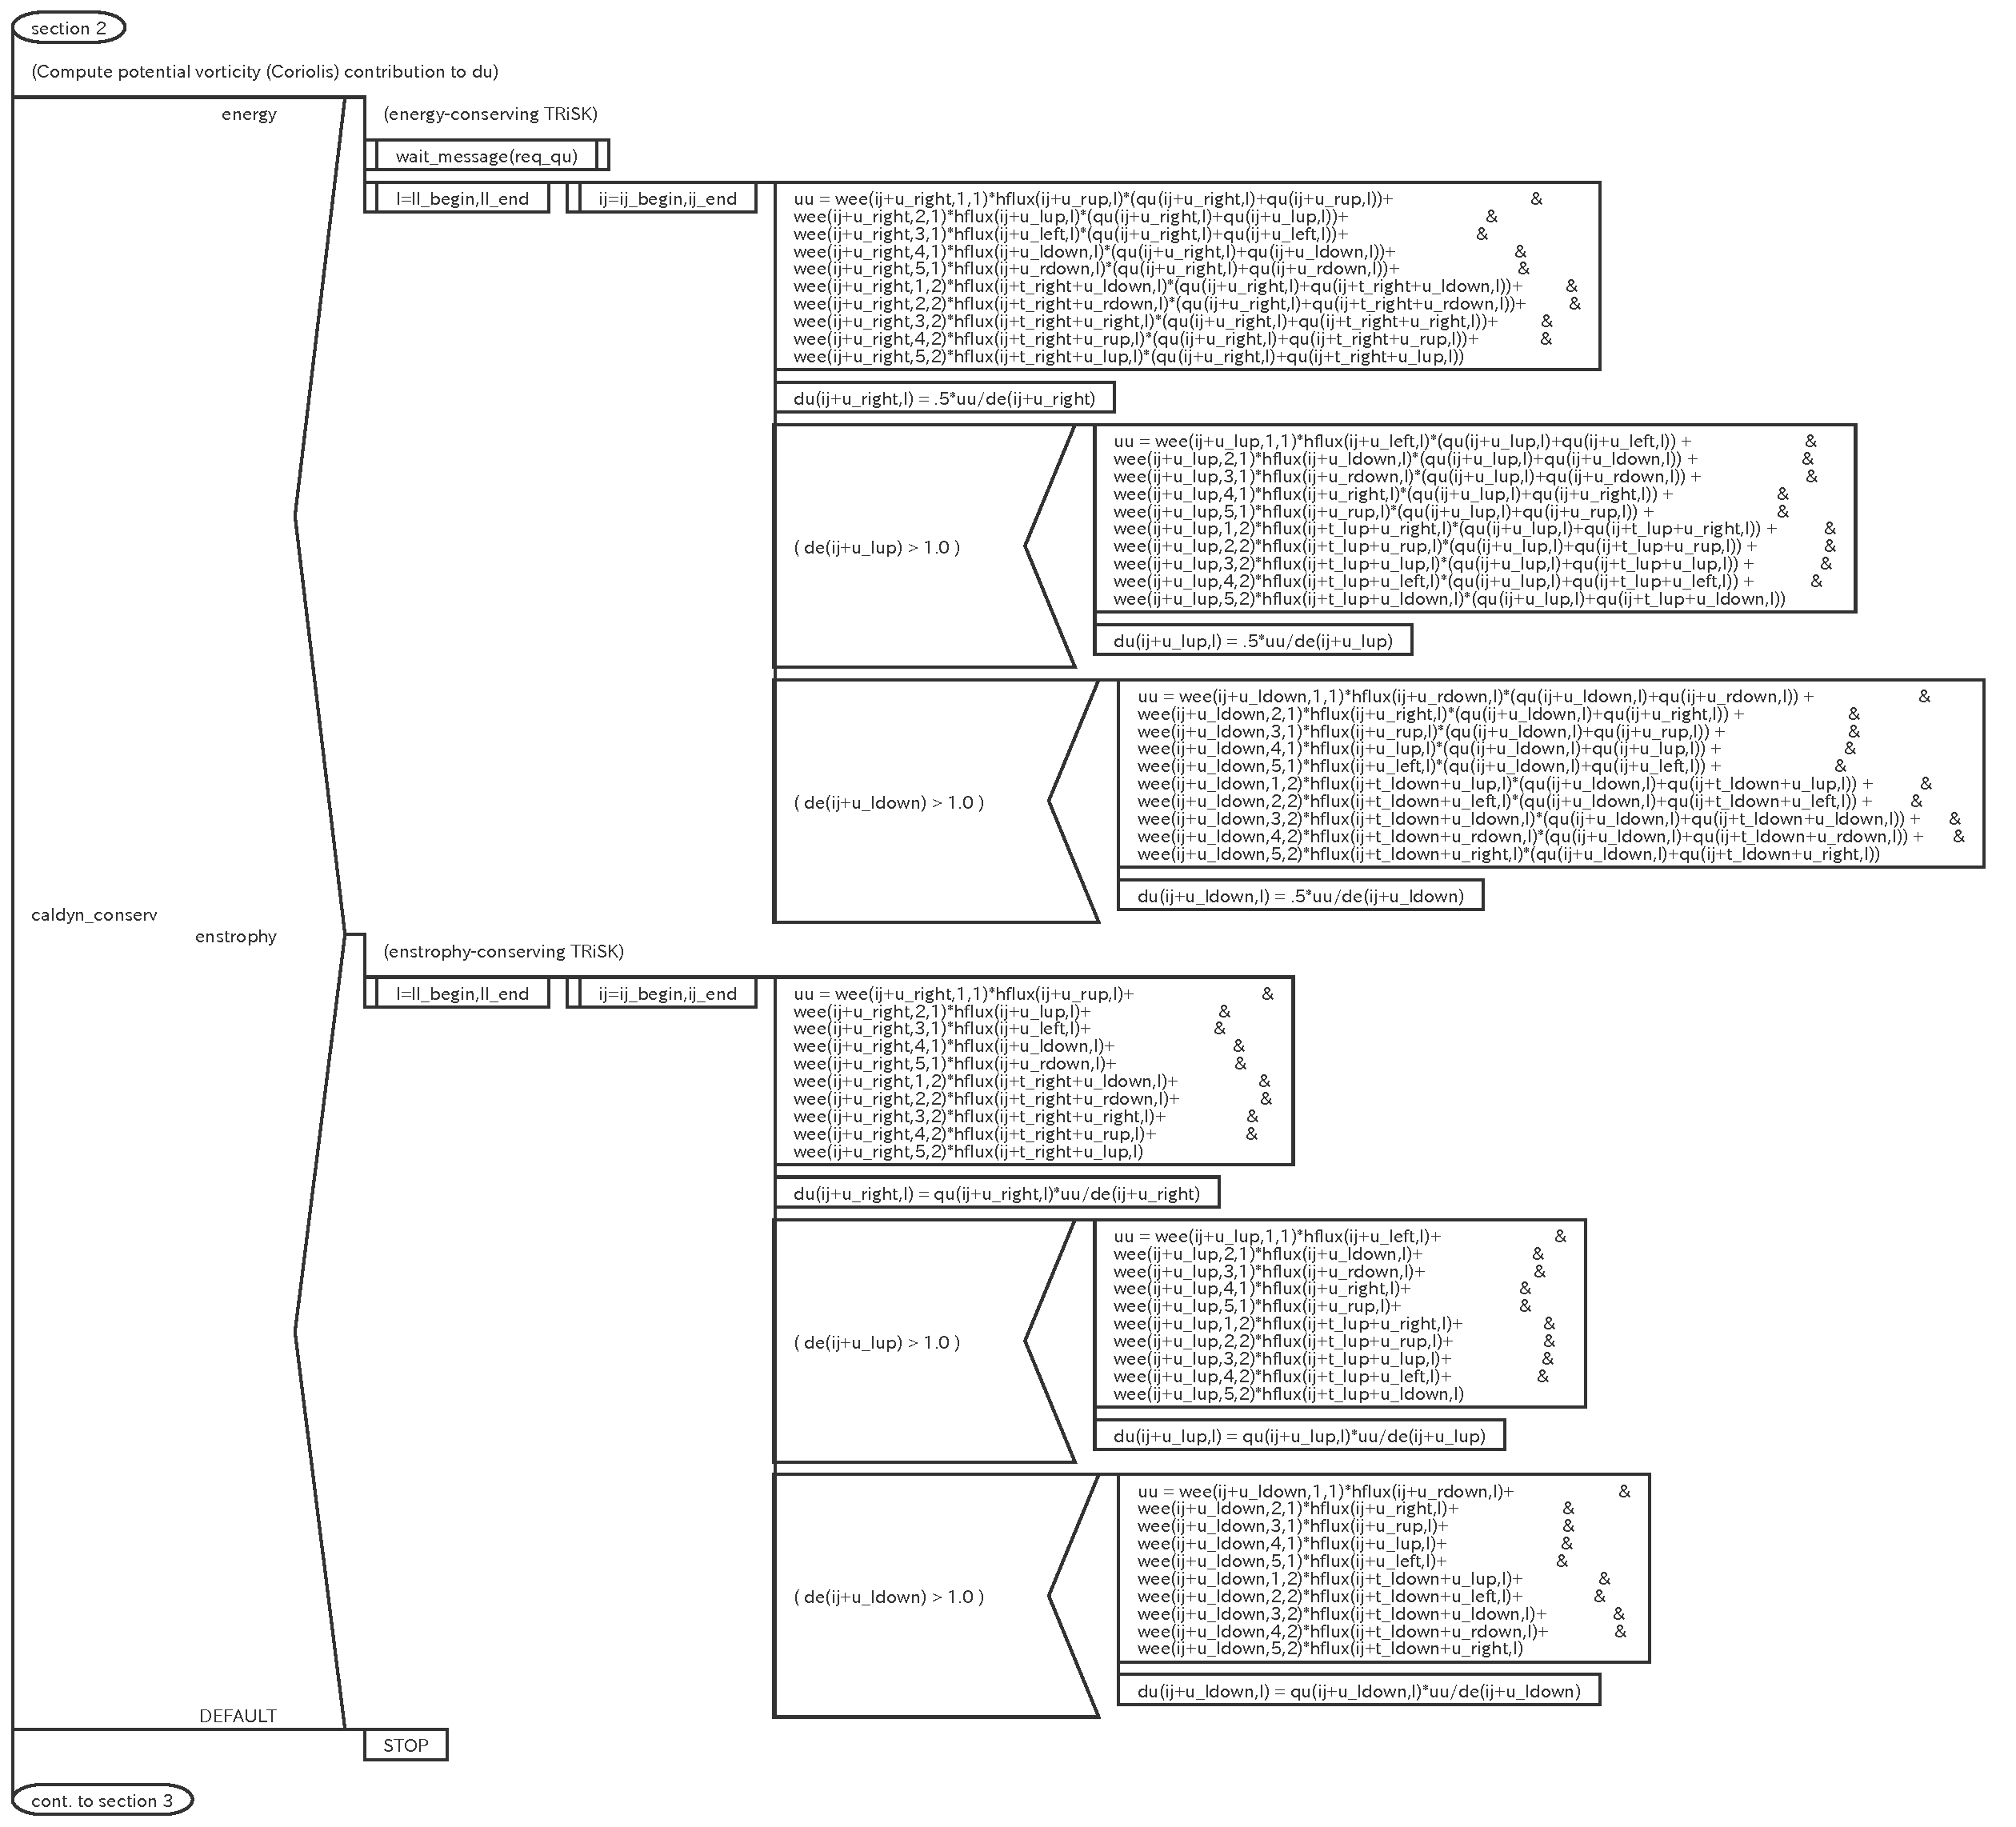
\includegraphics[scale=.4]{figs/caldyn_horiz_sec2.pdf}
 \caption{PAD of \src{compute_caldyn_horiz(2)}}\label{f:pad_comp_caldyn_horiz_2}
\end{figure}

The last section (\autoref{f:pad_comp_caldyn_horiz_3}) calculates Bernoulli term
first, then adds gradients of it and Extern functions to \src{du}.
%
Here Bernoulli term is sum of kinetic energy and geopotential.
%
Note that \src{boussinesq} is set as \src{.true.} in this kernel
package, Exner function \src{pk} is calculated in advance to calculate
Bernoulli term \src{berni}.

\begin{figure}[tbp]
\centering
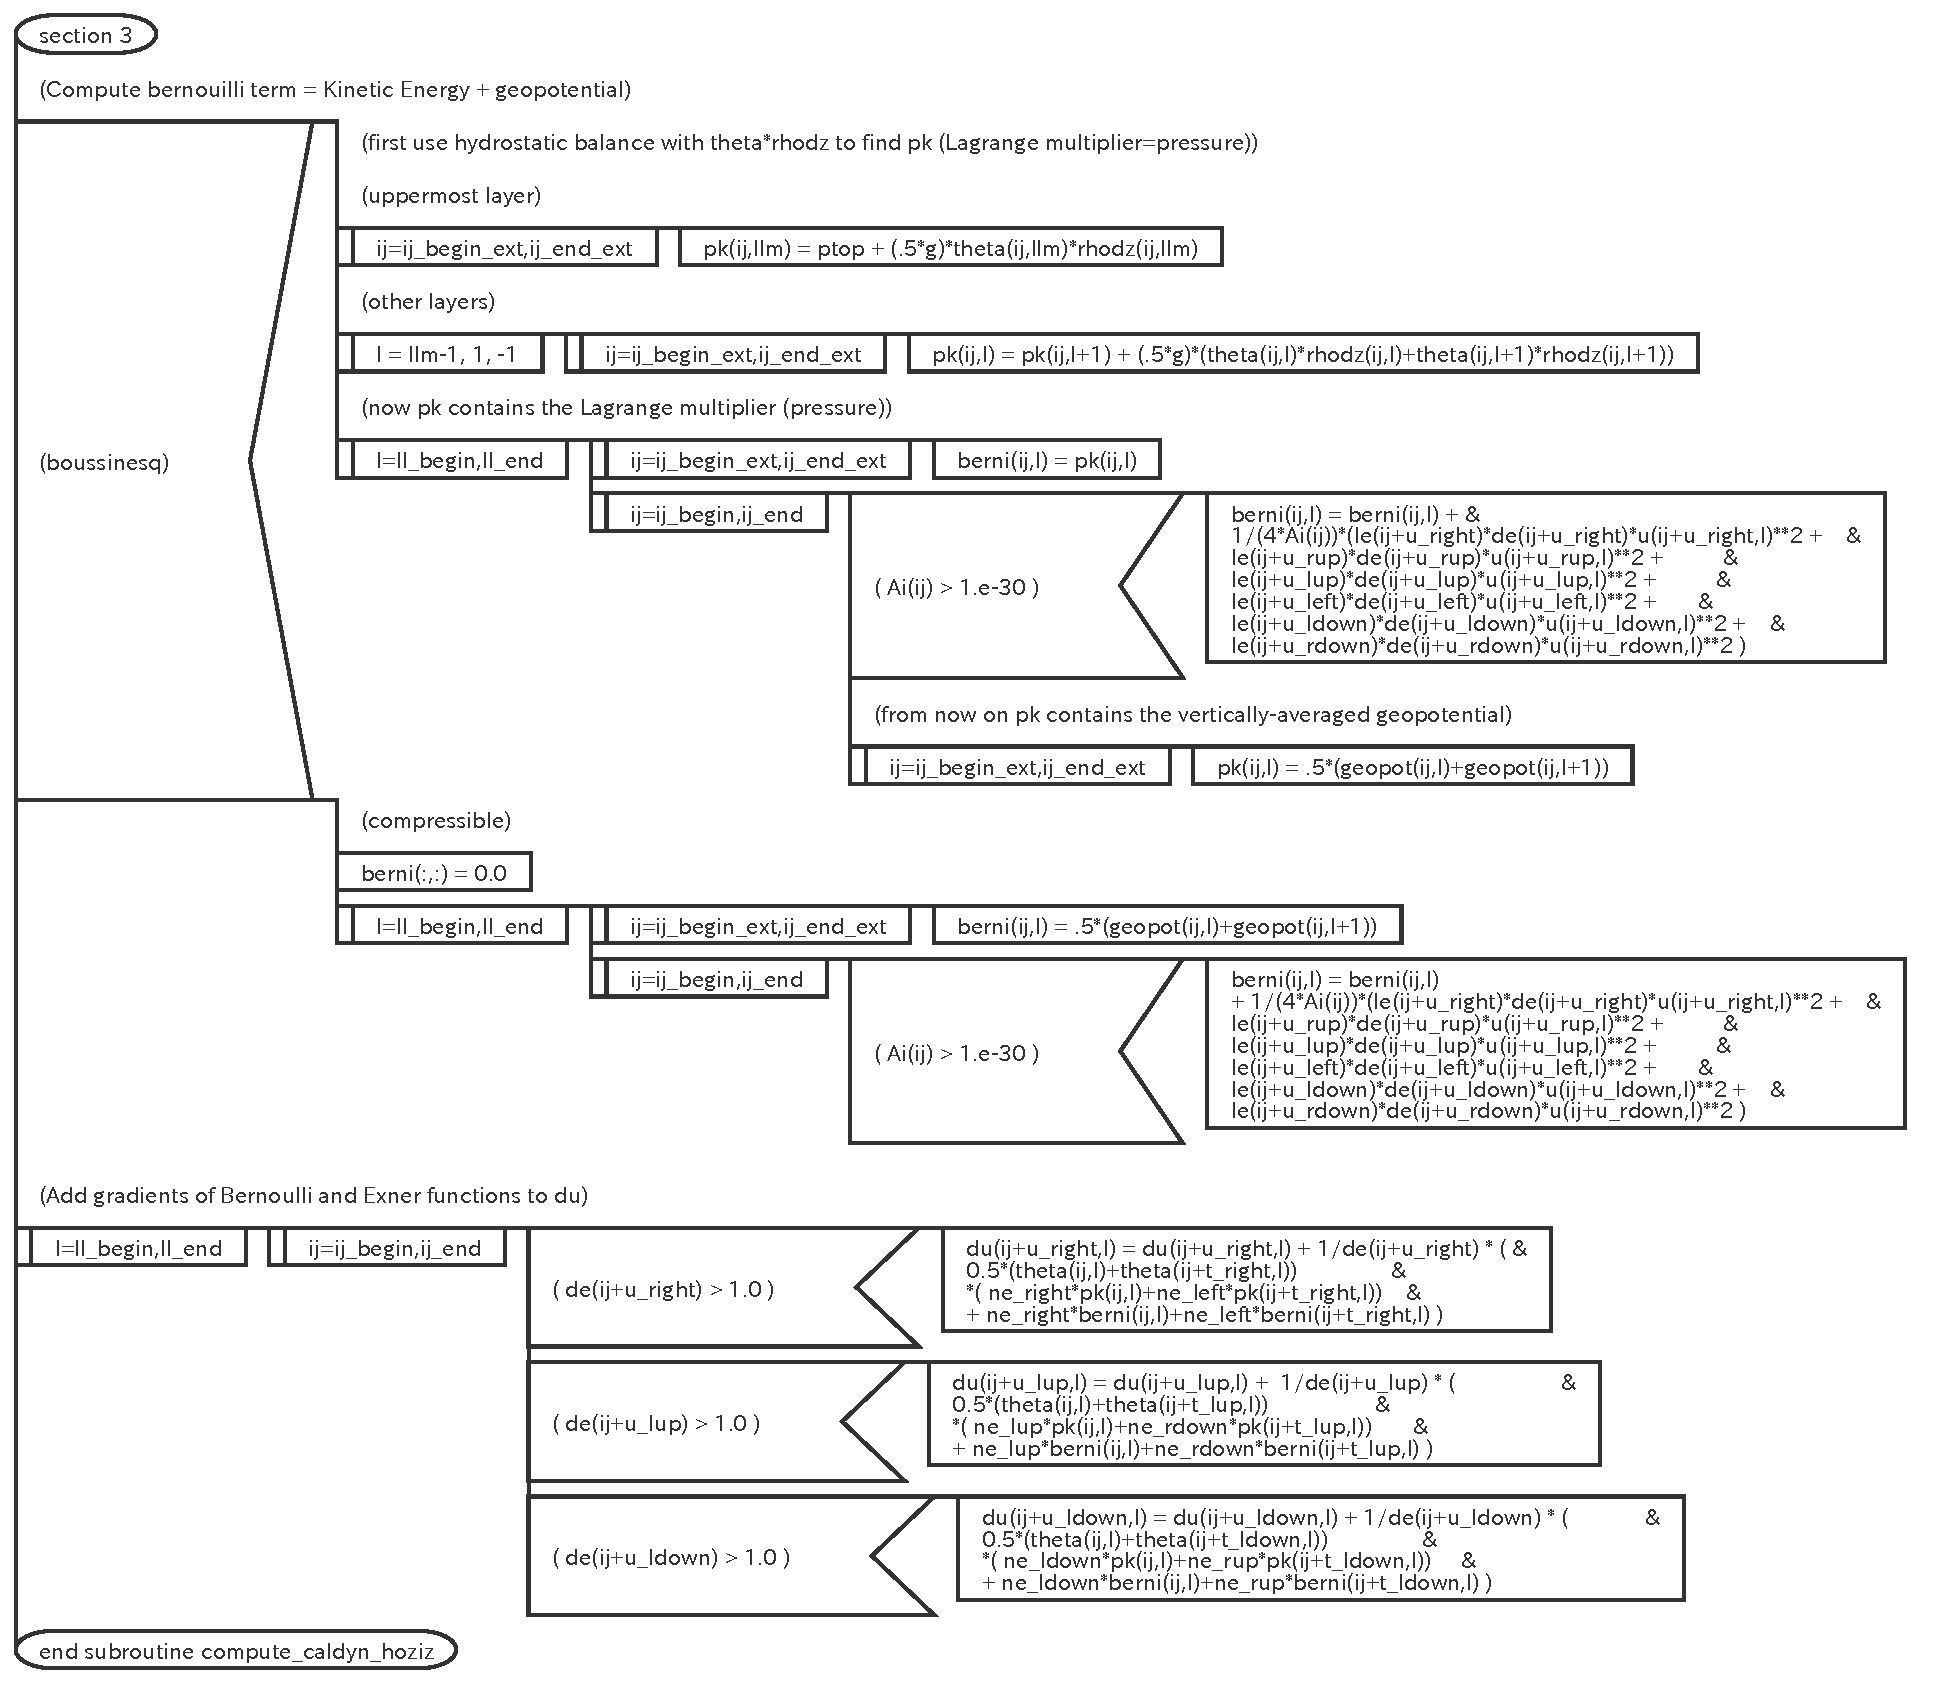
\includegraphics[scale=.5]{figs/caldyn_horiz_sec3.pdf}
 \caption{PAD of \src{compute_caldyn_horiz(3)}}\label{f:pad_comp_caldyn_horiz_3}
\end{figure}

\clearpage


\subsection{Input data and result}

Input data file is prepared and you can download from official server using
\file{data/download.sh} script.
%
This data file is created by original \DYNAMICO\footnotemark with
Held-Suarez case parameter set included in the original source archive.
%
\footnotetext{with slight modification by AICS.}
%
Max/min/sum of input/output data of the kernel subroutine are output as
a log.
%
Below is an example of \src{$IAB_SYS=Ubuntu-gnu-ompi} case.

\begin{LstLog}
 [KERNEL] comp_caldyn_horiz
 *** Start  initialize
                iim, jjm, llm:    23    25    19
             ij_begin, ij_end:    48   528
     ij_begin_ext, ij_end_ext:    24   552
             ll_begin, ll_end:     1    19
        t_right, t_rup, t_lup:     1    23    22
     t_left, t_ldown, t_rdown:    -1   -23   -22
        u_right, u_rup, u_lup:     0  1173   575
     u_left, u_ldown, u_rdown:    -1  1150   553
           z_rup, z_up, z_lup:   598     0   597
     z_ldown, z_down, z_rdown:   -23   575   -22
               caldyn_conserv:     1
                   boussinesq:     F
                            g:     9.80000000
 +check[pk_prev         ] max=  1.0014594722514462E+03,min=  0.0000000000000000E+00,sum=  6.9872296819747351E+06
 +check[hflux_prev      ] max=  0.0000000000000000E+00,min=  0.0000000000000000E+00,sum=  0.0000000000000000E+00
 +check[convm_prev      ] max=  0.0000000000000000E+00,min=  0.0000000000000000E+00,sum=  0.0000000000000000E+00
 +check[dtheta_rhodz_pre] max=  0.0000000000000000E+00,min=  0.0000000000000000E+00,sum=  0.0000000000000000E+00
 +check[du_prev         ] max=  3.4399140149818440E-03,min= -3.0658810374294527E-03,sum=  5.5109794763703335E-01
 +check[le              ] max=  1.3457165724385556E+05,min=  0.0000000000000000E+00,sum=  1.6031419146648201E+08
 +check[Ai              ] max=  3.4618288017294556E+10,min=  0.0000000000000000E+00,sum=  1.7746401564746273E+13
 +check[de              ] max=  4.5171816240714993E+06,min=  0.0000000000000000E+00,sum=  4.7785815753077912E+08
 +check[Av              ] max=  4.1228713627140027E+11,min=  0.0000000000000000E+00,sum=  3.2428753277257527E+13
 +check[Wee             ] max=  5.9893054722291683E-01,min= -5.8540209553487599E-01,sum=  2.4695023837951297E+01
 *** Finish initialize
 *** Start kernel
 ### check point iteration:           1
 ### Input ###
 +check[u               ] max=  4.1278968179782127E-01,min= -4.1278968179782127E-01,sum=  1.6791131703073393E+01
 +check[rhodz           ] max=  1.2306877011993038E+03,min=  0.0000000000000000E+00,sum=  5.3979591836733194E+06
 +check[qu              ] max=  1.0339537867296609E-06,min= -8.4408169682701225E-07,sum=  3.9419811615778674E-04
 +check[theta           ] max=  8.0139914420291746E+02,min=  0.0000000000000000E+00,sum=  3.8582633571973117E+06
 +check[geopot          ] max=  3.8250620498369227E+05,min=  0.0000000000000000E+00,sum=  1.1718001851963627E+09
 +check[pk_prev         ] max=  1.0014594722514462E+03,min=  0.0000000000000000E+00,sum=  6.9872296819747351E+06
 +check[hflux_prev      ] max=  0.0000000000000000E+00,min=  0.0000000000000000E+00,sum=  0.0000000000000000E+00
 +check[convm_prev      ] max=  0.0000000000000000E+00,min=  0.0000000000000000E+00,sum=  0.0000000000000000E+00
 +check[dtheta_rhodz_pre] max=  0.0000000000000000E+00,min=  0.0000000000000000E+00,sum=  0.0000000000000000E+00
 +check[du_prev         ] max=  3.4399140149818440E-03,min= -3.0658810374294527E-03,sum=  5.5109794763703335E-01
 ### Output ###
 +check[pk              ] max=  1.0014594722514462E+03,min=  0.0000000000000000E+00,sum=  6.9872296819747351E+06
 +check[hflux           ] max=  3.1805763161244854E+07,min= -2.8604204589892026E+07,sum=  2.4131331333014986E+08
 +check[convm           ] max=  1.0361970643226587E-03,min= -1.0359249303947807E-04,sum= -1.5233533963107249E-01
 +check[dtheta_rhodz    ] max=  3.2251351666935379E-01,min= -3.3676276308628725E-02,sum= -5.3720539414185993E+01
 +check[du              ] max=  3.4404317002518906E-03,min= -3.0804630348046005E-03,sum=  5.5048589972605033E-01
 ### final iteration:        1000
 ### Validation : grid-by-grid diff ###
 +check[pk              ] max=  0.0000000000000000E+00,min=  0.0000000000000000E+00,sum=  0.0000000000000000E+00
 +check[hflux           ] max=  0.0000000000000000E+00,min=  0.0000000000000000E+00,sum=  0.0000000000000000E+00
 +check[convm           ] max=  0.0000000000000000E+00,min=  0.0000000000000000E+00,sum=  0.0000000000000000E+00
 +check[dtheta_rhodz    ] max=  0.0000000000000000E+00,min=  0.0000000000000000E+00,sum=  0.0000000000000000E+00
 +check[du              ] max=  0.0000000000000000E+00,min=  0.0000000000000000E+00,sum=  0.0000000000000000E+00
 *** Finish kernel
\end{LstLog}

Check the lines below \src{``Validation : grid-by-grid diff''} line,
that shows difference between calculated output array and
pre-calculated reference array.
These should be zero or enough small to be acceptable.
%
There are sample output log files in \file{reference/}
in each kernel program directory, for reference purpose.

\subsection{Sample of performance result}

Here's an example of the performance result part of the log output.
Below is an example executed with the machine environment described in \autoref{s:measuring_env}.
%
Note that in this program kernel part is iterated 1000 times.

\begin{LstLog}
 *** Computational Time Report
 *** ID=001 : MAIN_comp_caldyn_horiz           T=     0.876 N=   1000
\end{LstLog}
